\chapter{Validation de la méthodologie AMIS sur un cas expérimental}

Dans ce chapitre, nous appliquons l'algorithme AMIS à un problème STE avec des données d'observations réelles issues d'une campagne expérimentale de mesures. Nous présentons dans un premier temps le contexte de la campagne, puis nous détaillons l'approche méthodologique ainsi que les résultats obtenus. Le contenu de ce chapitre reprend les travaux illustrés dans \cite{Rajaona2015}.

\section{Contexte: l'expérience FFT07}

La campagne expérimentale \textit{FUSION Fields Trials 2007} (FFT07) fût conçue et menée en 2007 par la \textit{Defense Threat Reduction Agency} (DTRA), une agence du Département de la Défense (DoD) des Etats-Unis dont la mission principale est axée autour de la prévention et de la protection vis-à-vis des risques NRBC.\\

Le but de FFT07 était de constituer une base de données météorologiques et de mesure de concentration issues d'une série de tests, ou \textit{trials}, chacun d'entre eux consistant en un rejet de gaz traceur sur une zone fortement instrumentée du site militaire de \textit{Dugway Proving Ground}, dans le désert de l'Utah.\\
Certains éléments de cette base de données ont été transmises à plusieurs équipes de recherche, chacune ayant pour tâche d'estimer au mieux les paramètres du terme source de chacun des \textit{trials} fournis (voir \cite{Platt2010}, \cite{Annunzio2012b}, et \cite{Singh2014} pour des exemples d'utilisation).\\

L'expérience FFT07 a été formatée pour étudier l'impact à courte portée des rejets de gaz traceur: le domaine considéré est un carré de 500 mètres de côté. Plusieurs configurations de rejet ont été utilisées, chacune caractérisant un \textit{trial} distinct par:
\begin{itemize}
	\item la période du jour où le rejet a eu lieu,
	\item la vitesse du vent et sa direction,
	\item la classe de stabilité atmosphérique,
	\item le nombre de sources ayant simultanément émis un rejet (1, 2 ou 3); \\
	\item dans le cas d'une source unique, le type du rejet: continu ou instantané.
\end{itemize}

L'acquisition des données s'est faite via un réseau de 100 capteurs à photo-ionisation (\textit{digital photoionization detectors}, ou digiPID), répartis en un maillage uniforme régulier sur l'ensemble du domaine. Ces capteurs sont situés à 50m les uns des autres, et à une hauteur de 2m du sol. La fréquence d'acquisition des concentrations est relativement élevée (50Hz): dans notre étude, nous avons réduit la dimension du vecteur d'observation en effectuant un moyennage sur des fenêtres de 10s afin que les calculs puissent se faire dans des temps raisonnables sans pour autant déplorer une perte significative d'information (voir figure \ref{fig_AE_3}).

\begin{figure}[h!]
	\centering
	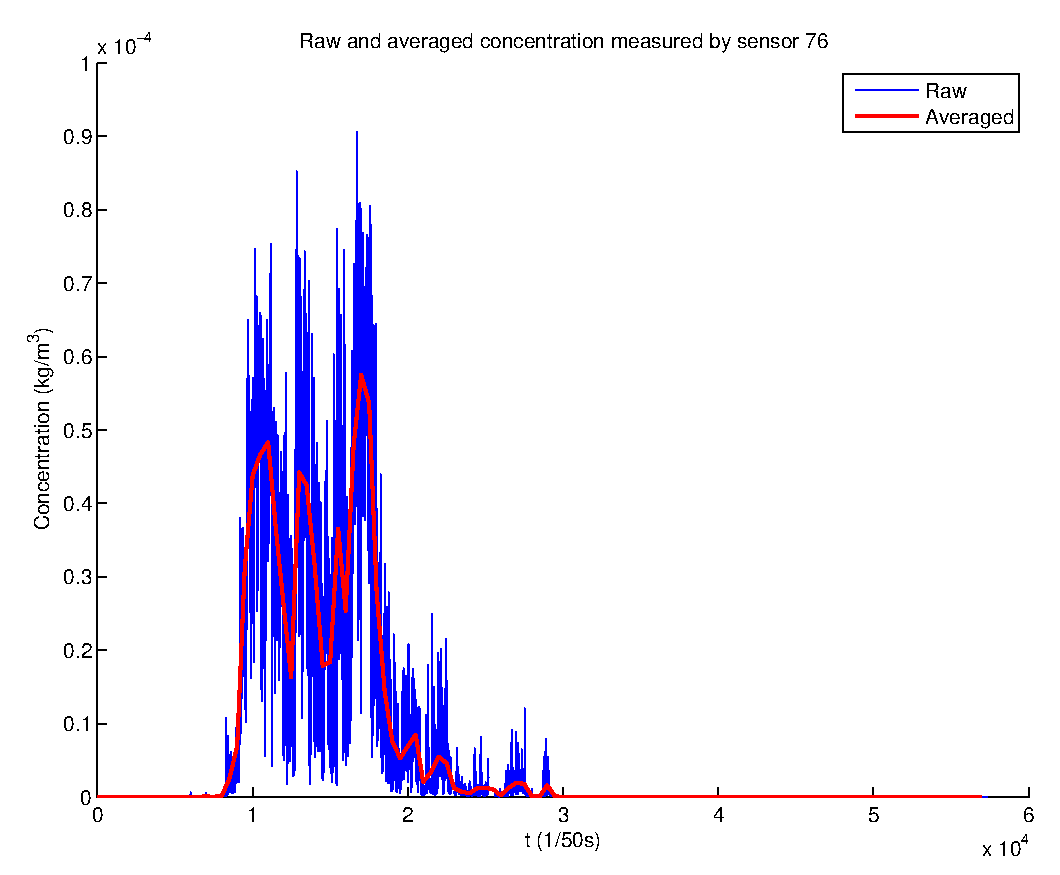
\includegraphics[scale=0.65]{moyennage_concentrations}
	\caption{Concentrations brutes (en bleu) et concentrations moyennées (en rouge) sur une fenêtre glissante de 10s. }
	\label{fig_AE_3}
\end{figure}


L'expérience FFT07 étant un outil de validation, le domaine d'étude comprend beaucoup plus de capteurs que dans un cas standard, où le domaine est moins instrumenté. Afin d'envisager un cas réaliste tout en conservant une quantité suffisante de données d'observation à traiter, nous avons choisi de limiter le nombre de capteurs exploitables à 25 (voir figure \ref{fig_AE_4}).

\begin{figure}[h!]
	\centering
	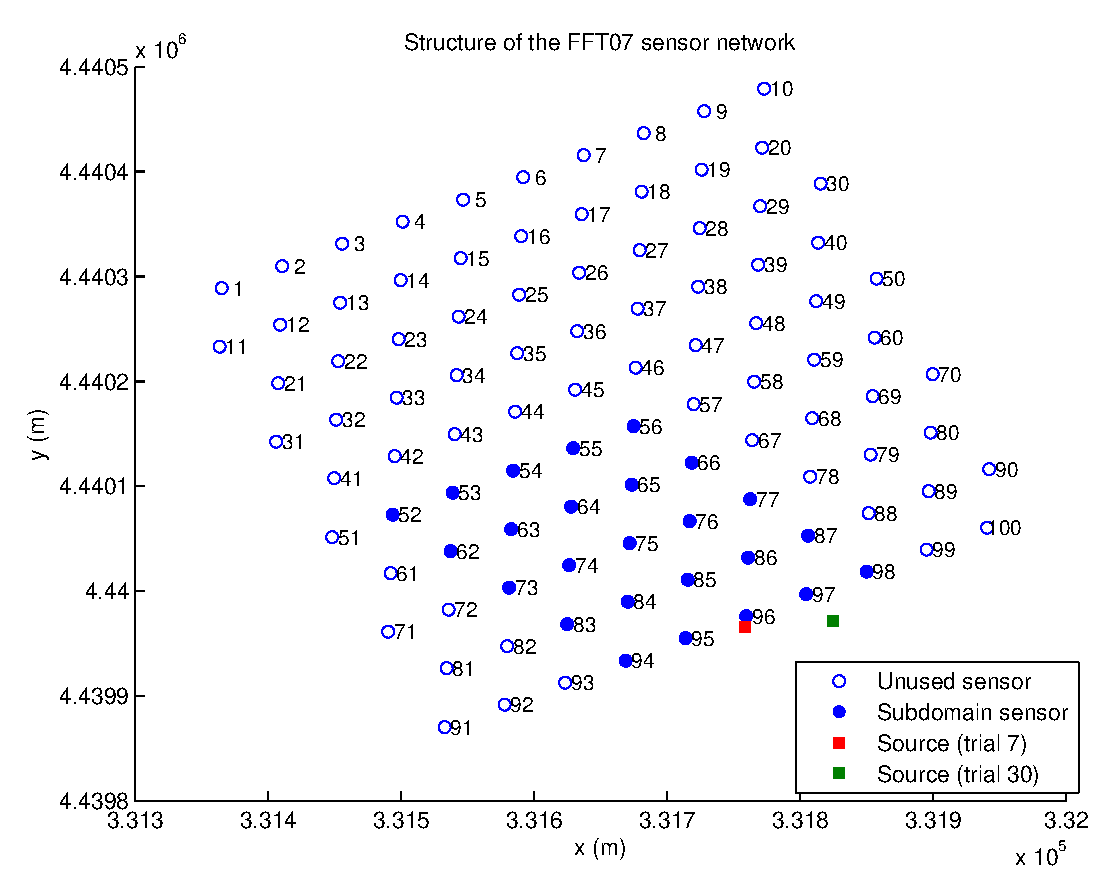
\includegraphics[scale=0.65]{FFT07_capteurs}
	\caption{Choix du sous-réseau de 25 capteurs utilisé dans notre étude.}
	\label{fig_AE_4}
\end{figure}

Dans notre cas, nous travaillons avec les configurations issues des \textit{trials} 7 et 30: 
\begin{itemize}
	\item Dans un premier temps, nous simulons à l'aide d'un modèle de dispersion les concentrations mesurées aux capteurs pour chaque \textit{trial},
	\item Nous effectuons ensuite la validation expérimentale à l'aides des concentrations réelles obtenues pour le \textit{trial} 7.
\end{itemize}



\section{Formulation bayésienne du problème STE}

\subsection{Modèle de données et vraisemblance}

Nous considérons ici une source localisée en un point $\PosSource = (x_s, y_s, z_s)$ de l'espace et caractérisée par un profil de rejet $\VecQSource$. Pour les besoins de la modélisation, ce dernier est discrétisé en $T_s$ échéances d'émission $t'_1, \cdots, t'_{T_s}$, l'intervalle entre deux échéances consécutives demeurant strictement identique. On peut ainsi définir $\VecQSource$ comme une succession de paliers d'émissions constantes suivant les intervalles temporels définis par:

\begin{equation}
\forall n \in \{2, \cdots, T_s\}, ~\Delta t'_n = t'_{n} - t'_{n-1}
\label{eq_def_delta_t}
\end{equation}


On suppose que les observations sont définies par des mesures de concentration en un nombre fini de points $ \PosCapteur^{(1)}, \cdots, \PosCapteur^{(N_c)}$ du domaine, qui constituent les positions d'un réseau de $N_c$ capteurs. On considère que les capteurs et la source se situent à la même hauteur, ce qui permet de n'étudier la position de la source que sur deux dimensions, autrement dit écrire $\PosSource = (x_s, y_s)$. Les mesures fournies par ces capteurs sont données suivant une discrétisation temporelle donnée, chaque capteur délivrant ainsi une valeur de concentration à chacun des instants d'observation $t_1, \cdots, t_{T_c}$.




 La concentration $\obs_{i,j}$ fournie par le $i$-ème capteur à la position $\PosCapteur^{(i)}$ et à l'échéance d'observation $t_j$ est alors modélisée par l'équation suivante: 
 
\begin{equation}
\obs_{i,j} = \sum\limits_{n=2}^{T_s}q(\Delta t'_n)\MatC_{i,j}(\PosSource, \Delta t'_n) + \varepsilon_{i,j}
\label{eq_AE_2}
\end{equation}

Le premier terme de l'équation \eqref{eq_AE_2} représente à la concentration moyenne obtenue par la superposition des $T_s$ rejets sur les différents intervalles d'émission $\left\{\Delta t'_n\right\}_{2\leq n \leq T_s}$et pondérés par les quantités émises $\left\{q(\Delta t'_n)\right\}_{2 \leq n \leq T_s}$ associées. Ainsi, $\MatC_{i,j}(\PosSource, \Delta t'_n)$ désigne la concentration moyenne observée par le $i$-ème capteur à la position $\PosCapteur^{(i)}$ et à l'échéance d'observation $t_j$ si un rejet unitaire aurait été produit sur l'intervalle $\Delta t'_n$ par une source située à la position $\PosSource$. Enfin, $\varepsilon_{i,j}$ représente le terme regroupant toutes les sources d'erreur présentées au paragraphe §\ref{ss_erreurs}.\\

Il est possible de réécrire l'équation \eqref{eq_AE_2} sous la forme matricielle suivante:

\begin{equation}
\VecObs = \MatC(\PosSource)\VecQSource + \VecErreur
\label{eq_AE_3}
\end{equation}
qui n'est autre que l'équivalent de l'équation \eqref{eq_relation_SR_non_parametrique}. $\VecObs \in \mathbb{R}^{N_cT_c}$ est un vecteur où toutes les observations de concentration sont concaténées sous la forme suivante : 

\begin{equation}
\VecObs = \left(\obs_{1,1}, \obs_{1,2}, \cdots, \obs_{1,T_c}, \obs_{2,1}, \cdots, \cdots, \obs_{N_c,T_c}\right)^T
\label{eq_AE_3_plus}
\end{equation}

$\VecErreur \in \mathbb{R}^{N_cT_c}$ est un vecteur d'erreur qui suit, comme présenté à l'équation \eqref{eq_bruit_obs}, une loi normale centrée de matrice de covariance $\MatR \in \mathbb{R}^{N_cT_c \times N_cT_c}$. De plus, on considère que ce vecteur de bruit affecte les observations de façon indépendante et identiquement distribuée (i.i.d.): par conséquent, la matrice $\MatR$ est diagonale:


\begin{equation}
\MatR = 
\begin{pmatrix}
\diagentry{\varObs}\\
&\diagentry{\varObs}\\
&&\diagentry{\xddots}\\
&&&&\diagentry{\varObs}\\
&&&&&\diagentry{\varObs}\\
\end{pmatrix}
\label{eq_AE_covariance_obs}
\end{equation}

Le terme $\MatC(\PosSource) \in \mathbb{R}^{N_cT_c \times T_s}$ est la matrice source-récepteur suivante:

\begin{equation}
\MatC(\PosSource) = 
\begin{pmatrix}
\MatC_{1,1}(\PosSource, \Delta t'_1) & \MatC_{1,1}(\PosSource, \Delta t'_2)  & \cdots & \MatC_{1,}(\PosSource, \Delta t'_{T_s}) \\ 
\MatC_{1,2}(\PosSource, \Delta t'_1) & \MatC_{1,2}(\PosSource, \Delta t'_2)  & \cdots & \MatC_{1,2}(\PosSource, \Delta t'_{T_s}) \\
\vdots & \vdots &  & \vdots \\
\MatC_{1,T_c}(\PosSource, \Delta t'_1) & \MatC_{1,T_c}(\PosSource, \Delta t'_2)  & \cdots & \MatC_{1,T_c}(\PosSource, \Delta t'_{T_s}) \\
\MatC_{2,1}(\PosSource, \Delta t'_1) & \MatC_{2,1}(\PosSource, \Delta t'_2)  & \cdots & \MatC_{2,1}(\PosSource, \Delta t'_{T_s}) \\
\vdots & \vdots &  & \vdots \\
\vdots & \vdots &  & \vdots \\
\MatC_{N_c,T_c}(\PosSource, \Delta t'_1) & \MatC_{N_c,T_c}(\PosSource, \Delta t'_2)  & \cdots & \MatC_{N_c,T_c}(\PosSource, \Delta t'_{T_s}) \\
\end{pmatrix}
\label{eq_AE_4}
\end{equation}

Si on note $\VecTheta = (\PosSource, \VecQSource)$ le vecteur des paramètres caractérisant le terme source, la règle de Bayes permet d'écrire la définition de la loi a posteriori de $\VecTheta$ : 

\begin{equation}
p(\VecTheta | \VecObs) = \dfrac{p(\VecObs | \VecTheta)p(\VecTheta)}{p(\VecObs)}
\label{eq_AE_1}
\end{equation}

Comme expliqué au paragraphe \ref{paragraphe_paradigme_bayesien}, on cherche à estimer cette loi a posteriori à un facteur multiplicatif près, l'équation \eqref{eq_AE_1} devient alors:

\begin{equation}
p(\VecTheta | \VecObs) \propto p(\VecObs | \VecTheta)p(\VecTheta)p(\VecObs)
\label{eq_AE_1_prop}
\end{equation}

Comme on connaît la nature gaussienne du vecteur d'erreur, on peut alors définir la vraisemblance des observations $\VecObs$ sachant un terme source donné $\VecTheta$:

\begin{equation}
p(\VecObs | \VecTheta) = \prod\limits_{i=1}^{N_c} \prod\limits_{j=1}^{T_c}\mathcal{N}\left(\obs_{i,j} \middle\vert \MatC_{i,j}(\PosSource)\VecQSource, \varObs\right)
\label{eq_AE_5}
\end{equation}

\subsection{Choix des lois a priori}

\subsubsection{Position de la source}

On considère que la source est forcément contenue dans les limites du domaine spatial $\mathcal{D}$ considéré, mais qu'elle peut se situer en n'importe quel point de ce domaine. En termes probabilistes, cela se traduit par une loi a priori uniforme sur la position $\PosSource$ de la source:

\begin{equation}
p(\PosSource) = \mathcal{U}_\mathcal{D}(\PosSource)
\label{eq_AE_7}
\end{equation}


\subsubsection{Profil d'émission}

Comme expliqué dans \cite{Winiarek2011}, la pratique la plus courante consiste à choisir un a priori gaussien pour le vecteur $\VecQSource$, qui s'écrit alors:

\begin{equation}
p(\VecQSource) = \mathcal{N}\left(\VecQSource \middle \vert \VecMeanQ, \MatCovQ\right)
\label{eq_AE_8}
\end{equation}

Dans \cite{Bocquet2008}, il est expliqué que l'hypothèse gaussienne sur $\VecQSource$ entraîne potentiellement des incohérences physiques telles que des valeurs d'émissions négatives. Cependant, une telle hypothèse demeure fréquemment utilisée dans la littérature, et conduit à des résultats satisfaisants (voir par exemple \cite{Issartel2003}) ainsi qu'une meilleure flexibilité quant à la quantification des connaissances a priori sur le type de rejet étudié. Par exemple, si on sait d'avance que le rejet se fait à un débit relativement faible, alors il est possible d'ajuster les valeurs de la diagonale de la matrice de covariance en y mettant des quantités faibles. \\

Il est toutefois possible d'atténuer les effets indésirables de l'hypothèse gaussienne sans avoir à changer la nature de la loi de probabilité a priori de $\VecQSource$, nous verrons comment cela est possible dans le prochain paragraphe.


\section{Marginalisation du profil d'émission}

\subsection{Principe}
La vraisemblance $p(\VecObs|\VecTheta)$ présentée à l'équation \eqref{eq_AE_5} est fortement non-linéaire, et la complexité de sa formulation rend impossible le calcul analytique de la loi a posteriori $p(\VecTheta | \VecObs)$. Afin de contourner ce problème, une solution consiste à exprimer cette loi a posteriori en fonction des différentes \textit{lois a posteriori marginales} dont elle dépend. \\

Par définition, la loi a posteriori $p(\VecTheta|\VecObs)$ peut s'exprimer en fonction de la loi jointe de $\VecTheta$ et $\VecObs$:

\begin{equation}
p(\VecTheta|\VecObs) = p(\PosSource, \VecQSource | \VecObs) = \dfrac{p(\PosSource, \VecQSource, \VecObs)}{p(\VecObs)}
\label{eq_conditionalite}
\end{equation}

En appliquant la règle du conditionnement en chaîne, ou \textit{chain rule}\footnote{La \textit{chain rule} permet d'exprimer une loi jointe sous la forme d'un produit de lois conditionnelles. Si on considère les $n$ variables aléatoires $X_1, \dots, X_n$, alors on a $p(X_1, \dots, X_n) = p(X_n|X_1, \dots, X_{n-1})p(X_{n-1}|X_1, \dots, X_{n-2})\dots p(X_2|X_1)p(X_1)$.}, sur le numérateur, on arrive à l'expression suivante:
\begin{equation}
p(\PosSource, \VecQSource | \VecObs) = p(\VecQSource | \PosSource, \VecObs)p(\PosSource | \VecObs)
\label{eq_AE_9}
\end{equation}
où $p(\VecQSource | \PosSource, \VecObs)$ et $p(\PosSource | \VecObs)$ sont les lois a posteriori marginales respectives du profil d'émission et de la position de la source. \\

\subsection{A priori gaussien et solution analytique}

Afin de passer de $p(\VecQSource)$ à $p(\VecQSource |\PosSource, \VecObs)$, on utilise une version statique des équations du \textit{filtre de Kalman}.\\

Le filtre de Kalman \cite{Kalman1961} est une méthode classique pour l'estimation d'état séquentielle dans le cas d'un phénomène qui n'est pas complètement observable et qui est défini par un système linéaire. Concrètement, il peut s'appliquer aux systèmes de la forme suivante:

\begin{equation}
\begin{split}
\VecQSource_t & = \bm{A}_n\VecQSource_{t-1} + \bm{b}_t\\
\VecObs_t & = \MatC_t(\PosSource) \VecQSource_t + \VecErreur_t
\end{split}
\label{eq_filtre_kalman_dynamique}
\end{equation}
où $\VecQSource_t$ représente l'état non-observable et $\VecObs_t$ le processus observable, en l'occurence les mesures de concentration, au temps $t$. L'opérateur $\bm{A}$ est une matrice de transition entre les états $\VecQSource_{t-1}$ et $\VecQSource_t$, et $\bm{b}_t$ est un bruit gaussien centré de variance connue.

 On suppose connu l'état initial $\VecQSource_0$ de $\VecQSource$,  autrement dit les paramètres $\bm{\mu}_{q_{0}}$ et $\bm{\Sigma}_{q_0}$ de sa loi a priori $p(\VecQSource_0)$ sont donnés. Le principe du filtre de Kalman consiste alors à calculer de façon récursive des estimateurs $\PostMeanQ_t$ et $\PostCovQ_t$ caractérisant l'état $\VecQSource_t$.\\
 
 Ici, notre problème est stationnaire, donc dans l'équation \eqref{eq_filtre_kalman_dynamique} on a $\bm{A}_n$ = $\bm{I}$ où $\bm{I}$ désigne la matrice identité, $\bm{b}_t = 0$ et la dépendance temporelle en $t$ disparaît: il n'y a qu'une unique étape de mise à jour, celle du passage de $p(\VecQSource)$ à $p(\VecQSource|\PosSource, \VecObs)$. Dans ce cas, les équations du filtre de Kalman permettent alors d'écrire les mises à jour suivantes:
 
 \begin{equation}
 \begin{split}
 \PostMeanQ & = \VecMeanQ + \MatK(\VecObs - \MatC(\PosSource)\VecMeanQ) \\
 \PostCovQ & = \MatCovQ - \MatK\MatC(\PosSource)\MatCovQ
 \end{split}
 \label{eq_filtre_kalman_statique}
 \end{equation}
 où $\MatK$ est la \textit{matrice de gain de Kalman} définie par:
 
 \begin{equation}
 \MatK = \MatCovQ\MatC(\PosSource)^T(\MatC(\PosSource)\MatCovQ\MatC(\PosSource)^T + \MatR)^{-1}
 \end{equation}
 
 
 
 
 
  De plus, si les observations sont soumises à un bruit gaussien et que la loi a priori $p(\VecQSource)$ est également gaussienne, alors le système \eqref{eq_filtre_kalman_dynamique} est gaussien, et par conséquent la loi a posteriori $p(\VecQSource|\PosSource, \VecObs)$ est également gaussienne, de moyenne $\PostMeanQ$ et de covariance $ \PostCovQ$ : 
  
  \begin{equation}
  p(\VecQSource|\PosSource, \VecObs) = \mathcal{N}(\VecQSource | \PostMeanQ, \PostCovQ)
  \label{eq_AE_13}
  \end{equation}
  
  Les paramètres $\PostMeanQ$ et $\PostCovQ$ sont ainsi obtenus de façon analytique (i.e. sans approximation) par les équations \eqref{eq_filtre_kalman_statique}. 

\subsection{Contrainte de positivité}

Dans le but d'assurer la positivité des valeurs d'émission de la source, une contrainte peut être appliquée sur les résultats de l'équation \eqref{eq_filtre_kalman_statique}, inspirée par les travaux de \cite{Simon2010}. Il s'agit d'utiliser une méthode permettant de restreindre les valeurs d'un vecteur d'état à un intervalle borné ou semi-borné prédéfini: pour cela, la densité de probabilité de ce vecteur d'état est tronquée suivant la contrainte que l'on cherche à appliquer. \\

Le processus de troncature est ainsi appliqué de façon séquentielle sur chaque composante de $\VecQSource$: on travaille ainsi à tronquer $T_s$ densités de loi univariées. Le détail de cette démarche est décrit par l'algorithme \ref{algo_PCO}, qui permet d'approximer la loi a posteriori marginale de $\VecQSource$ par : 

\begin{equation}
p^c(\VecQSource | \PosSource, \VecObs) = \mathcal{N}(\VecQSource | \PostMeanQ^c, \PostCovQ^c)
\label{eq_AE_16}
\end{equation}

\begin{algorithm}
	\DontPrintSemicolon
	\SetAlgoLined
	\SetKwInOut{Input}{Entrées}
	\SetKwInOut{Output}{Sorties}
	\Input{$\PostMeanQ$ et $\PostCovQ$}
	Initialisation: $\PostMeanQ^c=\PostMeanQ$ et $\PostCovQ^c=\PostCovQ$\;
	\For{$i=1:T_s$}{
		${\bm \gamma}_i=\begin{bmatrix}{\bf 0}_{1\times (i-1)} & 1  & {\bf 0}_{1\times (T_s-i)}\end{bmatrix}^T$\;
		Calculer ${\bm W}_i$ et ${\bm T}_i$ par la réduction de Jordan de $\PostCovQ^c$, i.e. ${\bm T}_i {\bm W}_i {\bm T}_i^T=\PostCovQ^c$\;
		Calculer ${\bm S}_i$ par l'orthogonalisation de Gram-Schmidt pour obtenir la matrice orthogonale ${\bm S}_i$ telle que $${\bm S}_i {\bm W}_i^{1/2} {\bm T}_i^T {\bm \gamma}_i=\begin{bmatrix}
		({\bm \gamma}_i^T \PostCovQ^c {\bm \gamma}_i)^{1/2} & 0 & \cdots & 0 
		\end{bmatrix} $$
		 $c_i=-\dfrac{{\bm \gamma}_i^T \PostMeanQ^c}{({\bm \gamma}_i^T \PostCovQ^c {\bm \gamma}_i)^{1/2}}$\;
		 $\mu_i=\dfrac{\phi(c_i)}{1-\Phi(c_i)}$ avec $\phi(\cdot)$ la densité de la loi normale centrée réduite, et $\Phi(\cdot)$ la fonction de répartition de la loi normale centreé réduite.\;
		 $\sigma^2_i=1-\mu_i(\mu_i-c_i)$\;
		 ${\bm z}_i=\begin{bmatrix}\mu_i & 0 & \cdots & 0 \end{bmatrix}^T$\;
		 ${\bm D}_i=\text{diag}(\sigma^2_i,1,\ldots,1)$\;
		Calculer les paramètres de la densité tronquée:
		\begin{align*}
		\begin{split}
		\PostMeanQ^c&={\bm T}_i {\bm W}_i^{1/2} {\bm S}_i ^T{\bm z}_i + \PostMeanQ^c\\
		\PostCovQ^c&={\bm T}_i {\bm W}_i^{1/2} {\bm S}_i^T {\bm D}_i  {\bm S}_i {\bm W}_i^{1/2} {\bm T}_i ^T \\
		\end{split}
		\end{align*}
	}
	\Output{$\PostMeanQ^c$ et $\PostCovQ^c$}
	\caption{Contrainte de positivité sur $\VecQSource$ par troncature de la densité de $p(\VecQSource | \PosSource, \VecObs)$}
	\label{algo_PCO}
\end{algorithm}

Notons qu'une telle procédure permet également d'optimiser le calcul de la vraisemblance marginale de la localisation de la source $p(\VecObs | \PosSource)$: celle-ci peut alors se calculer par le même procédé que celui employé dans l'équation \eqref{eq_AE_9}, et devient alors:

\begin{equation}
p^c(\VecObs | \PosSource) = \dfrac{p(\VecObs | \VecQSource, \PosSource)p(\VecQSource)}{p^c(\VecQSource | \PosSource, \VecObs)}
\label{eq_AE_17}
\end{equation}


 \begin{figure}[h]
 	 	\label{fig_AE_2}	
 	\centering
 	\begin{subfigure}[t]{0.5\textwidth}
 		\centering
		\includegraphics[width=1\textwidth]{ConstrainedFigure1.eps}
		\caption{}
 		\label{fig_AE_2_a}
 	\end{subfigure}%
 	\begin{subfigure}[t]{0.5\textwidth}
 		\centering
		\includegraphics[width=1\textwidth]{ConstrainedFigure2.eps}
		\caption{}
 		\label{fig_AE_2_b}
 	\end{subfigure}
 	\begin{subfigure}[t]{0.5\textwidth}
 		\centering
 		\includegraphics[width=1\textwidth]{ConstrainedFigure3.eps}
 		\caption{}
 		\label{fig_AE_2_c}
 	\end{subfigure} 

 	\caption{Illustration de l'application de la contrainte de positivité (en noir) sur les paramètres d'une distribution gaussienne bivariée (en rouge) dans trois cas distincts: sans corrélation (\ref{fig_AE_2_a}), avec corrélation négative (\ref{fig_AE_2_b}) et avec corrélation positive (\ref{fig_AE_2_c}).}
 \end{figure}

La figure \ref{fig_AE_2} résume bien le fonctionnement de l'algorithme \ref{algo_PCO}: la zone en noir représente la version tronquée aux valeurs positives de la distribution initiale (en rouge). 

\section{Localisation de la source avec l'algorithme AMIS}

Il s'agit ici d'étudier la loi a posteriori marginale $p(\PosSource | \VecObs)$ de la position de la source. Contrairement au profil d'émission, il est plus difficile d'obtenir une solution analytique pour caractériser cette distribution. Par conséquent, l'approche par simulation stochastique sera privilégiée, le but étant de chercher à approximer la distribution $p(\PosSource | \VecObs)$. \\

Nous appliquons l'algorithme AMIS décrit dans le chapitre 2 afin de localiser la source. Dans un cadre bayésien, la loi a posteriori marginale recherchée peut s'écrire à une constante multiplicative près, suivant la relation de proportionnalité suivante:

\begin{equation}
p(\PosSource | \VecObs) \propto p(\VecObs | \PosSource)p(\PosSource)
\label{eq_AE_20}
\end{equation}

La fonction de vraisemblance $p(\VecObs | \PosSource)$ est définie par l'équation \eqref{eq_AE_5} (ou \eqref{eq_AE_17} si on choisit d'appliquer la contrainte de positivité), et la loi a priori $p(\PosSource)$ par l'équation \eqref{eq_AE_7}. 

\subsection{Choix de la loi de proposition}

L'algorithme AMIS requiert une loi de proposition paramétrique qui soit suffisamment flexible pour pouvoir envisager plusieurs configurations d'initialisation, qu'il s'agisse de partir d'une répartition uniforme des particules ou d'une distribution favorisant une zone cible pré-définie. Suivant la logique développée dans \cite{Cappe2008}, on choisit ainsi une mixture de $D$ distribution gaussiennes bivariées:

\begin{equation}
\varphi_{(\alpha,\nu)}(\PosSource) = \sum\limits_{d=1}^D \alpha_d \varphi_d(\PosSource | \nu_d)
\label{eq_AE_21}
\end{equation}
où les $\alpha_d$ sont les facteurs d'influence de chacune des composantes de la mixture, et $\nu_d$ représente le vecteur des paramètres de la $d$-ième composante, telle que : 
\begin{equation}
\varphi_d(\PosSource | \nu_d) = \mathcal{N}(\PosSource | \VecMu_d, \MatSigma_d)
\label{eq_AE_21_bis}
\end{equation}
avec $\VecMu_d \in \mathbb{R}^2$ et $\MatSigma_d \in \mathbb{R}^{2\times2}$. Pour la suite, on choisit $D=4$, ce qui est suffisant pour bien couvrir le domaine sans pour autant avoir de recouvrement entre les particules échantillonnées depuis différentes composantes. Le choix des paramètres initiaux, en particulier celui de $\MatSigma_d$, permet de régler la surface couverte par chacune des composantes afin d'obtenir une répartition relativement homogène des particules, illustrant une absence de connaissance a priori sur une localisation potentielle de la source (voir figure X).

 \begin{figure}[h!]
 	\label{fig_init_amis}	
 	\centering
 	\begin{subfigure}[t]{0.5\textwidth}
 		\centering
 		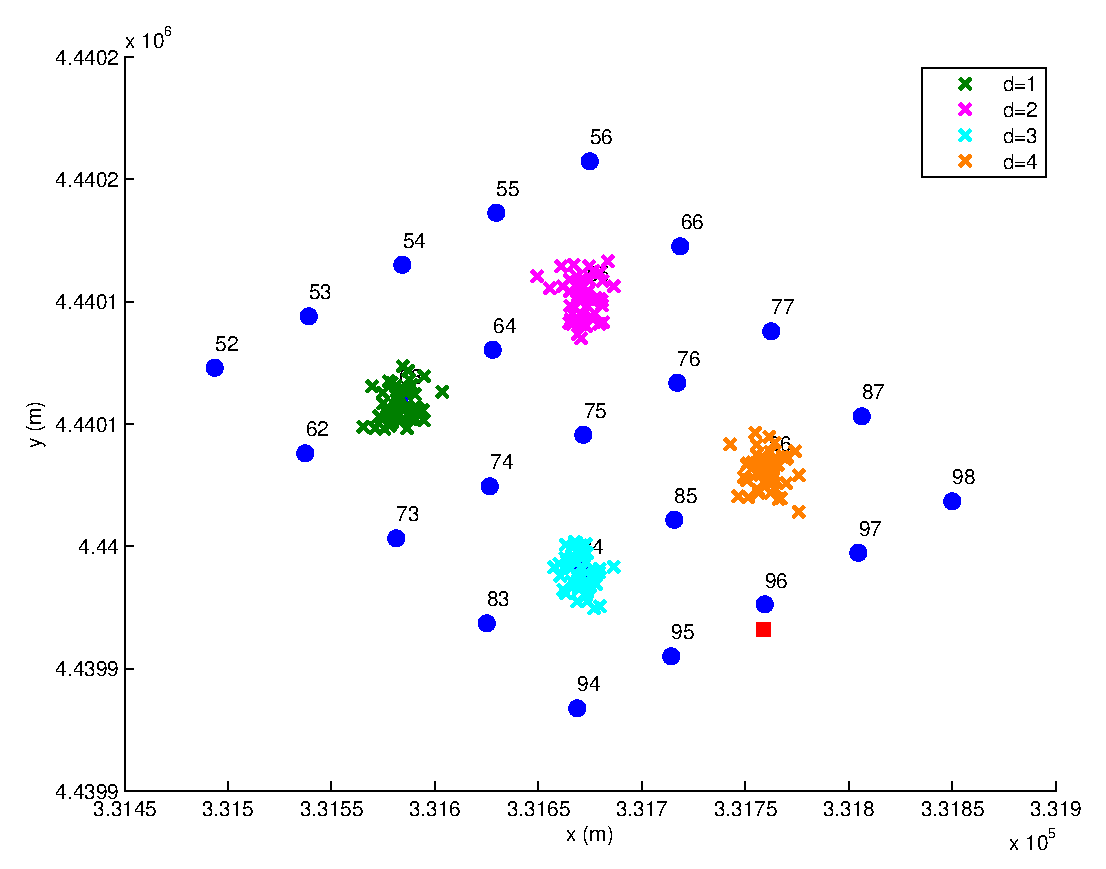
\includegraphics[width=1\textwidth]{init_amis_bad.eps}
 		\caption{$\MatSigma_d = 
 			\begin{pmatrix}
 			50 & 0 \\
 			0 & 50
 			\end{pmatrix}$}
 		\label{init_amis_bad}
 	\end{subfigure}%
 	\begin{subfigure}[t]{0.5\textwidth}
 		\centering
 		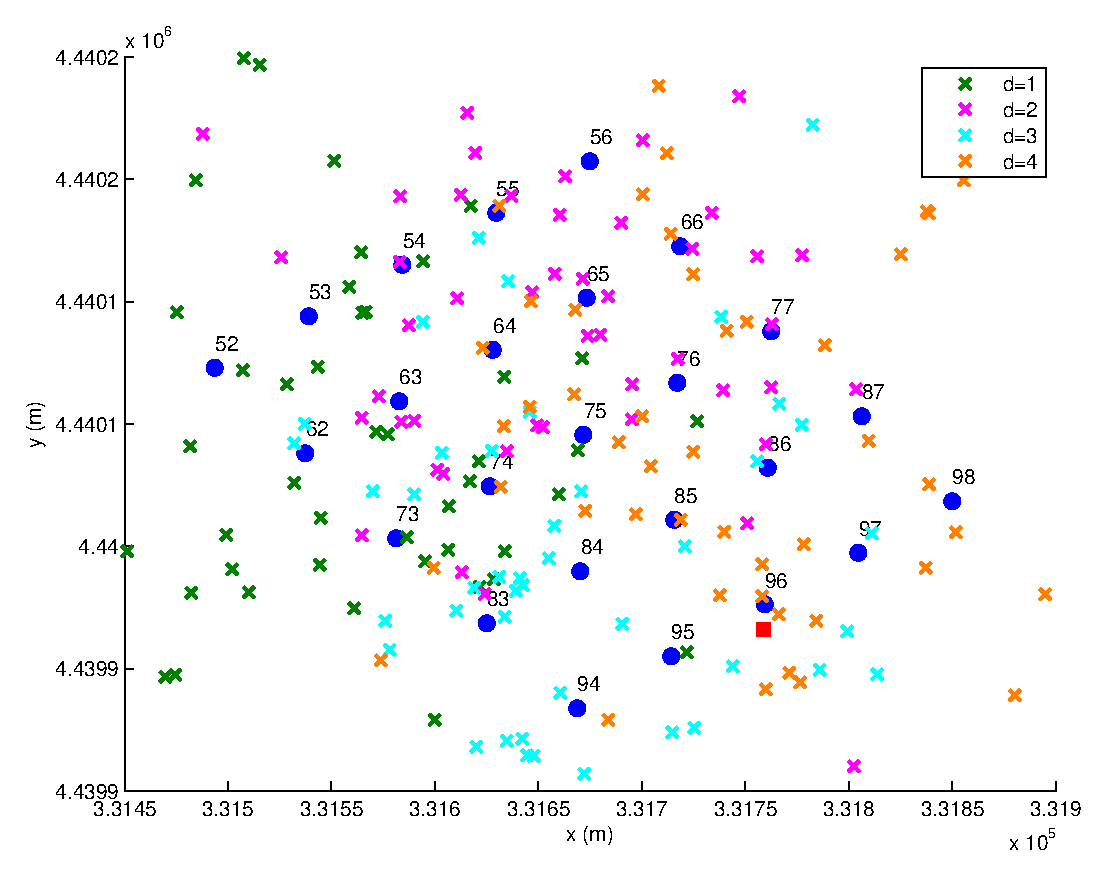
\includegraphics[width=1\textwidth]{init_amis_good.eps}
 		\caption{$\MatSigma_d = 
 			\begin{pmatrix}
 			5000 & 0 \\
 			0 & 5000
 			\end{pmatrix}$}
 		\label{init_amis_good}
 	\end{subfigure}
 	
 	\caption{Exemples d'initialisation de l'AMIS avec $D=4$ composantes pour la loi de proposition: un bon choix des $\MatSigma_d$ permet un tirage homogène sur le domaine (\ref{init_amis_good}) tandis qu'une covariance trop faible ne permettra pas d'explorer tout le domaine (\ref{init_amis_bad}).}
 \end{figure}


\section{Description du modèle de dispersion à bouffées gaussiennes}

\section{Résultats}